\chapter*{Introduction}
\addstarredchapter{Introduction}
\markboth{Introduction}{Introduction}
\label{chap:introduction}
\begin{mdframed}[hidealllines=true,backgroundcolor=lightgray!20]
\section*{Résumé}
Les émissions de $CO_2$ anthropogènes contribuent au réchauffement climatique par des phénomènes physiques aujourd'hui bien compris \cite{change2007physical}. Le secteur du transport aérien est en particulier responsable du 2 $\%$  du total des émissions provoqués par l'activité humaine (\cite{icao2016environmental}) mais ce chiffre est destiné à augmenter dans les prochaines années (\cite{terrenoire2019contribution}).  Pour cette raison des mesures concrètes pour la réduction des émissions de $CO_2$ s'appliqueront aux nouveaux avions à partir de 2020 et aux avions en production à partir de 2019 \cite{national2016commercial}. Si l'on classe les avions par leurs capacité on peut s'apercevoir que les plus grands consommateurs de carburant sont les avions avec une capacité supérieure à 100 passagers \cite{yutko2011approaches,epstein2019considerations}. Cela implique que l'effort de recherche doit être dirigé sur la réduction des émissions de ces dispositifs. Ces avions sont souvent propulsés par des moteurs thermiques du type turbofan. Dans ces moteurs la poussée est fournie par une soufflante qui est entrainée dans sa rotation par une turbine. Pour réduire leur consommation de carburant, l'architecture de ces systèmes évolue vers des concepts à très haut taux de dilution (UHBR). Cela demande une réduction du diamètre du carter de la partie core (turbine proprement dite) et une augmentation du diamètre de la soufflante. L'intégration d'un tel moteur représente un défi technologique majeur. En effet due à sa géométrie les déformations moteur seront plus difficiles à contrôler en particulier la variations des jeux entre partie tournant et partie fixe du moteur. Ces jeux appelés "tip-clearance" peuvent en effet changer à cause du chargement appliqué au moteur à cause des manœuvres de l'avion. Cela a différentes conséquences néfastes sur son fonctionnement, entre autre l'augmentation de leur consommation de carburant \cite{lattime2002turbine}.  Ces moteurs sont souvent montés sous la voilure par un mât et couvert par une coque aérodynamique appelée nacelle. Les deux contribuent à la performance finale par différents phénomènes. Dans cette thèse on s'intéresse à l'impact que les raideurs de la structure primaire du mât et de la nacelle ont sur la performance moteur par leur impact sur les déformations moteurs et donc sur les "tip-clearance". Pour avoir une quantification de ces impacts la simulation par éléments finis a été utilisée. De plus pour pouvoir identifier des solutions innovantes, l'optimisation topologique a été considérée. Le but de cette optimisation structurale est d'identifier des structures ayant de performances optimales sous des chargements définis et ayant un budget en masse défini. Dans cette thèse on a en particulier considéré 2 familles d'approches: les approches dites Eulériennes et Lagrangiennes \cite{zhang2016lagrangian} selon la description faite de la solution. Si la solution est décrite par des champs de fonctions qui indiquent la présence où l'absence de matière dans chaque point de l'espace de design alors on parle d'approches Eulériennes. D'autre part si la solution est décrite par une assemblage de formes élémentaires qui peuvent changer de positions et de dimensions alors on parle d'approches Lagrangiennes. Les deux ont des avantages et des inconvénients que sont étudiés dans cette thèse. Pour réaliser cet étude et l'appliquer à un contexte industriel un cadre d'analyse par éléments finis et d'optimisation topologique a été développé. Pour cela différents défis techniques ont été soulevés:
\begin{enumerate}
\item Le traitement des modèles éléments finis industriels de moteur. 
\item Le géométrie de région de design quelconque.
\item La communication de maillages incohérents.
\item L'efficacité et la scalabilité des algorithmes considérés.
\item L'implémentation des contraintes en stress dans l'optimisation topologique. 
\item L'implémentation des approches Lagrangiennes.
\item L'introduction de composantes géométriques spécifiques au problème industriel. 
\end{enumerate} 
\end{mdframed}
\section*{Industrial context}
\marginnote{\textsl{Aviation $CO_2$ reduction challenge}}[1cm] 
Energy production and transportation nowadays rely on fossil fuel combustions such as coal, natural gas and oil. As a consequence, human activity contributes to the release of carbon dioxide ($CO_2$) and other greenhouse gases like methane, nitrous oxide and fluorinated gases. The physical phenomena that make the link between global warming and greenhouse gases anthropogenic emissions are well understood \cite{change2007physical}. Since the first industrial revolution, $CO_2$ has been the major contributor to global warming.
To face this situation, governments and private companies of all industrial sectors started working for the reduction of $CO_2$ emissions.
In 2016, the International Civil Aviation
Organization (ICAO) recalled that the aviation sector ‘accounts for under 2 $\%$ of the world’s annual $CO_2$ emissions' (\cite{icao2016environmental}). 
As commercial aviation keeps growing in term of revenue-passenger miles and cargo ton miles, $CO_2$ emissions are expected to increase \cite{terrenoire2019contribution} therefore actions to reduce them are urgent and need to be considered in the present. It is in fact expected that a new fuel economy standard will be incorporated in national rules to reduce both aircraft emissions and noise.
It will apply to new aircraft design in 2020 as well as to in-production type in 2023 \cite{national2016commercial}.\\
\begin{figure}[ht]
\centering
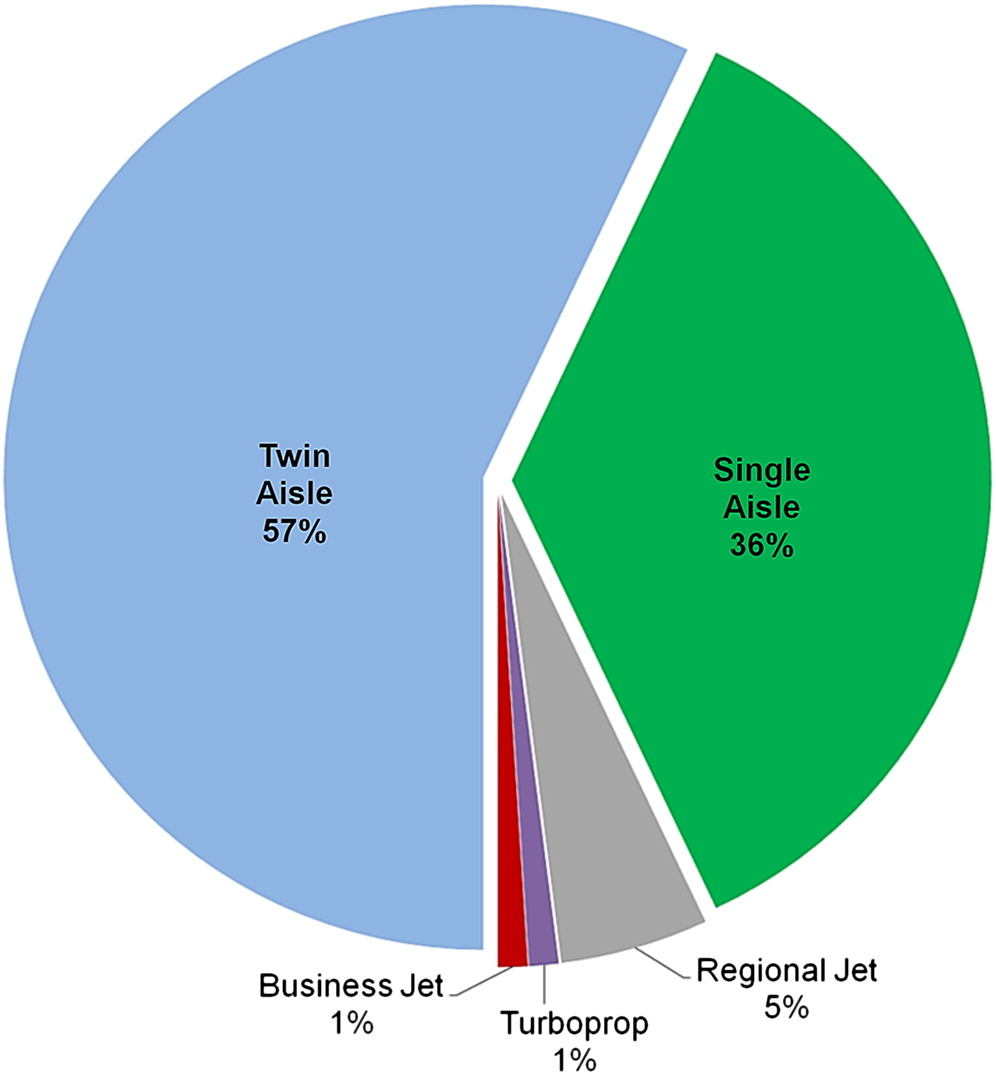
\includegraphics[width=8cm]{images/intro/figure2}
\caption{Global civil aviation fuel consumption. Source: \cite{yutko2011approaches,epstein2019considerations}}
\label{fig.intro1}
\end{figure}
Commercial aircraft can be organized in the following families:
\begin{itemize}
\item General aviation: fewer than 6 passengers
\item Commuter: fewer than 20 passengers
\item Regional: 30-100 passengers
\item Single-aisle: 100-200 passengers 
\item Twin-aisle: more than 200 passengers
\end{itemize}
In figure \ref{fig.intro1} we reported the distribution of global fuel consumption for each class \cite{yutko2011approaches}. It can be observed that more than 90 $\%$ of the $CO_2$ emissions from global commercial aircraft operations are generated by large aircraft. 
That is why single-aisle and twin-aisle are subjected to large research investments for their fuel consumption reduction.
\marginnote{\textsl{Propulsion integration airframe structures}}[1cm]
These families of aircraft are often propelled by turbofan engine (c.f. figure \ref{fig.intro2}).
\begin{figure}[!ht]
\centering   
 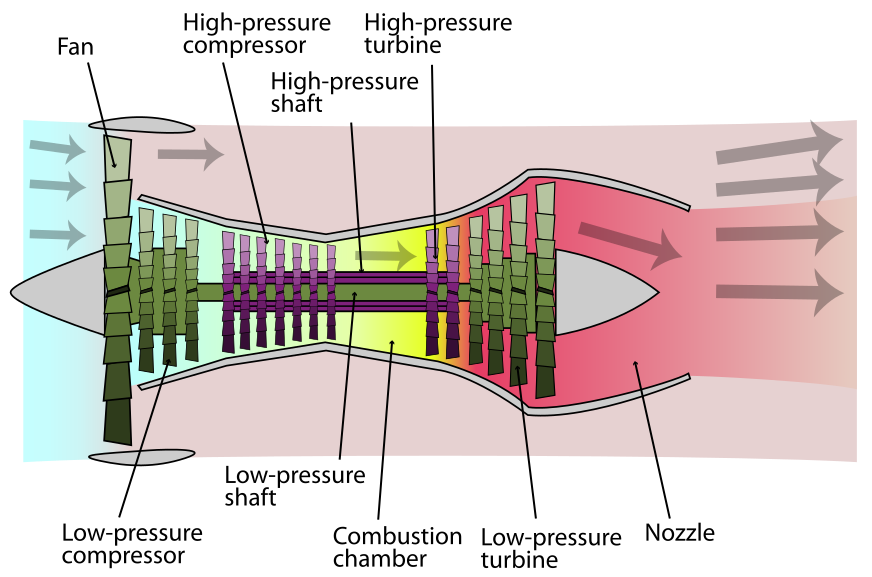
\includegraphics[width=0.75\textwidth]{images/intro/Turbofan_operation}
     \caption{Turbofan schematic representation. SOURCE: Wikipedia}
     \label{fig.intro2}
\end{figure}
This gas turbine engine is composed by a fixed casing and by several spools. Airflow passing through the fan and then in compressors, combustion chamber and turbines follows a Brayton cycle. Thanks to the excess of power produced by this cycle, the fan provides engine thrust. 
Engines on current turbofan-powered commercial aircraft are mounted on pylons, which keep the engines off the wings or fuselage in order to isolate the engine and airframe aerodynamic characteristics (c.f. figure \ref{fig.intro5}).
\begin{figure}[!ht]
	\centering   
	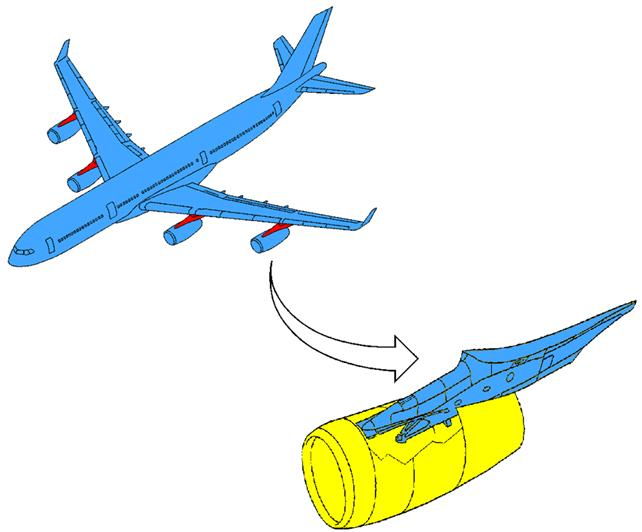
\includegraphics[width=0.75\textwidth]{images/intro/pylon_location}
	\caption{Commonly adopted pylon position in large turbofan propelled aircraft. Source: \cite{ASDM}} 
	\label{fig.intro5}
\end{figure}
The pylons must transmit the thrust loads from the engine to the airframe as well as convey all fluid and electrical
interconnections. 
\begin{figure}[!ht]
	\centering   
	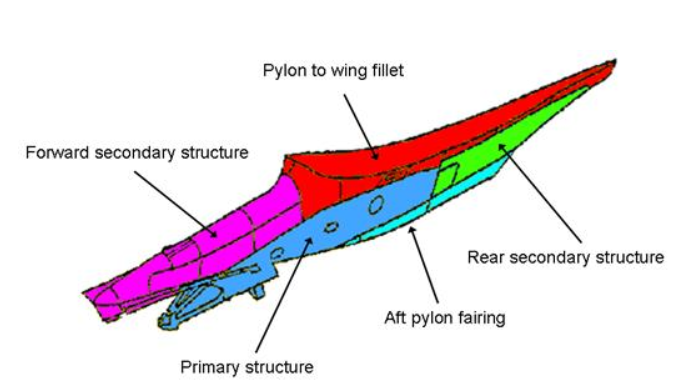
\includegraphics[width=0.75\textwidth]{images/intro/pylonA340}
	\caption{Pylon structure (A340 example). Source: \cite{ASDM}} 
	\label{fig.intro6}
\end{figure}
Among pylon substructures (c.f. figure \ref{fig.intro6}), primary structure transfers engine loads to the wing. This is ensured by a system of connections between pylon and engine or wing (so called engine and wing mounts respectively) and by the pylon torque box that joins these two. The engines are enclosed by fairings known as nacelles (c.f. figure \ref{fig.intro7}), which contain many of the subsystems
important to the operation of the aircraft such as the electrical generators. The nacelles also serve other purposes,
including aerodynamic fairing of the engine, conditioning of airflow into the engine, thrust reversing, and noise
attenuation. The aerodynamic, structural, and subsystem integration of the engine and nacelle with the airframe are
important to determine aircraft performance and optimum engine characteristics such as propulsor diameter and
fan pressure ratio. \clearpage
\begin{figure}[!ht]
	\centering   
	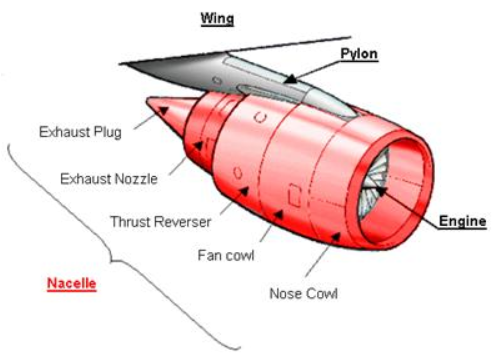
\includegraphics[width=0.75\textwidth]{images/intro/nacelle}
	\caption{Nacelle subsystems. Source: \cite{ASDM}} 
	\label{fig.intro7}
\end{figure}
\marginnote{\textsl{Increasing the Bypass Ratio}}[1cm]
To improve the existing propulsion efficiency several technologies are currently investigated \cite{national2016commercial}. One of those consists in increasing the so called bypass ratio. This is defined as the ratio between the airflow passing through the fan and then ejected from the fan nozzle (which mainly contributes to engine thrust) and the airflow passing through the combustion chamber (responsible for power generation).   
Increasing turbofan bypass ratio has the following consequences on design and performances:
\begin{itemize}
\item Fan diameter needs to be increased. As a consequence, the propulsion efficiency is also improved. In fact for the same level of thrust provided by the fan, outlet air velocity  can be reduced, consequently reducing losses and noise. 
\item Core diameter needs to be decreased. This is because aircraft propulsive efficiency is improved and that means that less power is demanded for the same level of engine thrust. Moreover this is also needed to improve thermodynamic efficiency when the temperature and pressure in the first stage of turbine are increased. \cite{national2016commercial}. 
\end{itemize}
Engine and integration design are challenged by these drivers for several reasons. \marginnote{\textsl{Tip-clearance variation challenge}}[1cm] Among others, such designs have to deal with larger engine deformations that can deteriorate the control of stator to rotor blade  tip clearances, defined as the radial gap between the rotor blade tips and the engine casing. In fact a larger engine will be subjected to larger loads and eventually to larger deformations. On top of that the center of gravity of the engine is moved forward possibly amplifying the effect of inertial loads. An appropriate sizing needs to be considered in order to avoid excessive closures or openings.
An abradable coat material is often applied to the engine casing. 
 This sacrificial material is often milled by the rotor due to engine deformations that can close these gaps. When this happens, the aerodynamic performance of the stage is reduced, increasing the overall engine specific fuel consumption. Moreover, to keep the same level of thrust, more fuel needs to be injected in the combustion chamber consequently increasing the temperature of outlet gas. Engine material can then be subjected to high temperature corrosion phenomena that reduce the engine time on wing \cite{lattime2002turbine}. In compressor stages these gaps have even more severe consequences since surge margin is reduced. This means that not only fuel consumption is affected, but also safety and engine operability \cite{benito20083d}. Also in the fan stage the openings reduce the propeller efficiency further impacting the specific fuel consumption.\\
\marginnote{\textsl{Tip-clearance drivers}}[1cm]  
Tip clearance variations in both compressor and turbine stages can be due to both  engine loads (propulsion induced) and flight loads. Engine loads include centrifugal, thermal,
internal engine pressure, and thrust loads. Flight loads
include inertial (gravitational), aerodynamic (external
pressure), and gyroscopic loads. Engine loads can
produce both axisymmetric and asymmetric clearance
changes (see Figures \ref{fig.intro3} and \ref{fig.intro4}). Flight loads produce
asymmetric clearance changes \cite{lattime2002turbine}. 
\begin{figure}[!ht]
\centering   
 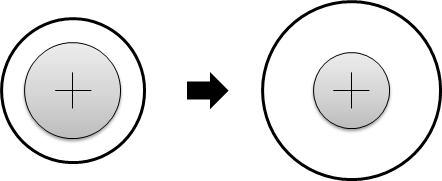
\includegraphics[width=0.5\textwidth]{images/intro/axisym_tip}
     \caption{Axisymmetric clearance variations} 
     \label{fig.intro3}
\end{figure}
\begin{figure}[!ht]
\centering   
 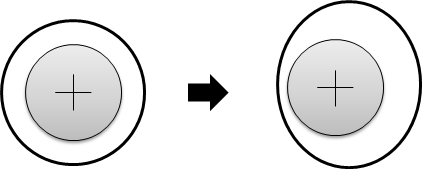
\includegraphics[width=0.5\textwidth]{images/intro/asym_tip}
     \caption{Asymmetric clearance variations} 
     \label{fig.intro4}
\end{figure}
Axisymmetric variations are mainly driven by engine rotor and stator sizing and by operating conditions. Nacelle and pylon are both linked to the engine. This means that their stiffness can have an impact on loads passing through each interface with the engine, therefore on the engine deformations. As a direct consequence pylon and nacelle design has an impact on tip clearance variation.\cite{lattime2002turbine}.  This contribution to the overall tip clearance variation in classic turbofan engine represents about a third of the total variation induced by other sources \cite{lattime2002turbine}. Nevertheless the relative importance of such contribution is still to be quantified for Ultra High Bypass Ratio (UHBR) architectures (Bypass ratio of the order of 30).\newpage
\marginnote{\textsl{A design problem}}[1cm] 
 The investigations that we want to conduct here, consist in studying how design choices made on:
 \begin{itemize}
 \item Engine outer casing main structure
 \item Engine to wing load path
 \item Nacelle and pylon main structure
 \end{itemize}
affect engine tip clearance variations in the context of UHBR architecture. For the aforementioned considerations such designs could be beneficial for both $CO_2$ emissions, engine life and safety. 
 In the determination of such a design one should be able to estimate the performance, in terms of tip clearance variation control and select a design considered 'best' among others.\\ 
 \marginnote{\textsl{Simulation driven design}}[1cm]
 Using only engineering considerations in the context of such complex phenomena could possibly be misleading or insufficient. For this reason an automated procedure, based on optimization algorithms in combination with a simulation model are proposed. A mathematical description of each configuration is then required and corresponding models should be available. In particular, structural optimization approaches deal with mechanical responses and often try to achieve the lightest or the stiffest design responding to some strength requirements on the solution. \\
 \marginnote{\textsl{Why Topology Optimization?}}[1cm] Depending on the design mathematical description, the optimal solution is more or less driven by the modeling choice made on the solution. In our industrial problem, assumptions made on the connectivity between pylon and engine can drive the solution to configurations that one cannot ensure to be optimal.  For this reason a way of considering a large spectrum of possible solutions is by addressing the problem in a topology optimization framework. 
\section*{Topology Optimization approaches}
 Topology optimization is a powerful tool that can be used to explore structural design. The inputs for topology optimization are the geometry of the design zone (i.e. a region in the space delimitating the structure), boundary conditions and materials. A structural model (often a Finite Element model) is generated to compute each configuration's responses. 
The formulation can then be stated, in the form of a non-linear constrained optimization problem. This means that a model response is selected as objective to be minimized or maximized and other responses are constrained.
For what concern the design variables, a general distinction can be made at this level:
\begin{itemize}
\item The design variables are associated to the presence or the absence of material, at a given point/element in the space. We refer to these approaches as Eulerian in this work \cite{zhang2016lagrangian} in reference to the continuum mechanics and the representation of displacements. In this first family we can find more common density based approaches \cite{bendsoe1989optimal,zhou1991coc,bendsoe1995optimization},  Level Set approach \cite{wang2003level,allaire2004structural} and ,  evolutionary approaches \cite{xie1993simple,xia2018bi}. 
\item The design variables are associated with geometric properties of features that are assembled to obtain the final solution. We refer to this second family as Lagragian or explicit approaches \cite{zhang2016lagrangian}. Classic examples are the Moving Morphable Components approach (MMCs) \cite{guo2014doing,guo2016explicit,zhang2016new,zhang2017new}, the Moving Morphable Voids (MMVs) \cite{zhang2017explicit}, the Geometry Projection Method (GP) \cite{bell2012geometry,norato2015geometryde,zhang2016geometry}, the Method of Moving Morphable
Bars (MMB) \cite{hoang2017topology} and  the Moving Node Approach (MNA) \cite{overvelde2012moving}. 
\end{itemize}
In both cases design variables are constrained by lower and upper bounds. Once that the optimization problem is stated, gradient based optimization algorithms are typically employed to improve an initial guess design. When a solution is determined, in both cases the solution has to be interpreted in terms of geometry, manufacturing technology and advanced design considerations. Further optimizations (shape and sizing) are often casted to obtain sized designs that respect reserve factors (i.e. safety factors). In \cite{zhu2016topology} one can find an up to date review of the most promising applications of topology optimization to aerospace structures. Topology optimization has shown its advantages for the design of aircraft parts like the wing internal primary structure \cite{eves2009topology,aage2017giga}, the wing-box, fuselage \cite{niemann2013use,singh2016topology} and of the pylon \cite{remouchamps2011application,xue2012structural}.  
\section*{PhD goals}
\marginnote{\textsl{Engine-wing load path determination}}[1cm]
As aforementioned the load path between engine and wing, is a contributor to engine performance and in particular fuel consumption. Note that there are larger contributors to the engines’ performances which are exclusively dependent on the engine manufacturer's design choices. However the engine's attachment to the wing and the resulting load path, is a significant contributor to the performance while being mainly a design choice of the aircraft manufacturer.
Physical intuition can be effective in this choice, only for very simple considerations. On the other hand to prevent complex phenomena like engine casing ovalization, physical intuition is often misleading. For this reason simulation should be used as an exploration tool to get rid of bad solutions and select promising configurations. To address such a complex problem, without making too strong hypotheses on the solution's connectivity, a topology optimization strategy is investigated in the present work. 
\marginnote{\textsl{Research axes}}[1cm]
In this PhD we seek to develop a topology optimization framework, initially intended to use Eulerian approaches and successively adapted for Lagrangian approaches to address this design problem. Eulerian approaches are able to represent organic designs that can be considered as reference solutions, even if not attainable by nowadays manufacturing technologies. Lagrangian approaches on the other hand make an assumption on the basic components that should compose the solution. For this reason their power of representation is restrained, but their advantage is their link with an explicit geometry representation. This can both decrease the overall optimization computational effort and the end to end design effort.
The following challenges should then be addressed in order to deal with the engine-to-wing attachment design problem:
\begin{enumerate}
\item Our framework should be able to deal with industrial engine finite element models allowing also the post-processing of tip clearance variations. Such models are often provided in industrial finite element software like Nastran or Abaqus. An efficient interface with such programs should be therefore provided.
\item Complex geometries of the design zone may require at least non uniform meshes. In fact due to aerodynamic needs and also to the kinematic interfacing with the engine and design region models, voxel meshes should be avoided.  
\item  Finite element simulations including inconsistent mesh interfaces between models should be allowed. The engine model being provided by the engine manufacturer comes in a given discretization. To avoid constraints on design region discretization the provided framework should be able to connect non consistent discretizations.
\item  Efficiency and scalability should be implementation drivers as the resolution of 3D topology optimization problems can quickly become prohibitive. In fact reducing finite element mesh size the computational burden associated with both analysis and optimization is increased. The provided framework should therefore employ adapted techniques for both.  
\item The possibility to consider stress based topology optimization. In fact most topology optimizations are concerned with  structural stiffness. On the other hand the stiffest design is not always the strongest. Dealing with stress problem is challenging and the provided framework should adopt appropriate techniques. 
\item The use of Lagragian approaches in topology optimization. A shortcoming of Eulerian approaches is their lack of an explicit control on the final solution geometry, often requiring human intervention and solution simplifications to provide an acceptable design. Lagrangian approaches provide an efficient solution to this issue and should therefore be provided by the proposed framework.
\item The introduction of explicit geometric constraints linked to the product to be designed. In fact another advantage of Lagrangian approaches is the possibility to use constitutive components that can make easier the determination of a manufacturing process for the solution. The proposed framework will allow this investigation.
\end{enumerate}
At the best of our knowledge at the beginning of this project there wasn't any industrial or academic framework that could provide a satisfactory answer to all these requirements. For this reason a novel topology optimization framework will be developed in this study.
The goal of this work can be resumed in this question:\\
\textit{Can we identify disruptive design features of engine pylon and mounts architecture that have an impact on tip clearance variations?} 
\\
The question was investigated by the development of a novel topology optimization framework that had to provide effective solutions to the aforementioned challenges.
%\marginnote{\textsl{Programming Language Considerations}}[1cm]
 %Nevertheless existing libraries for finite element analysis and topology optimization provide a baseline for the development of the proposed framework.
 %Some features considered in this framework are nevertheless unique and were developed from scratch. For this reason Matlab programming language was considered despite computational efficiency possible implications. 
\section*{Layout}
Our investigation can be divided in 3 large topics that we will cover in this manuscript, the finite element analysis, the Eulerian topology optimization approaches and the Lagrangian topology optimization approaches.
As a consequence the reminder of this work is organized as follows:
\begin{itemize}
\item \textbf{Chapter \ref{chap:1}} deals with challenges related to our design problem encountered in finite element analysis, state of the art approaches and proposed solutions.  The fundamentals of linear static analysis and finite element analysis are reviewed in section \ref{sec:1.1}. A representative use case engine finite element Model,  built for this work, is presented in subsection \ref{ssec1.2.1}. The post processing of tip clearances required to assess a performance analysis is also presented in subsection \ref{ssec1.2.2}.  In section \ref{sec1.3} some advanced techniques for the interface of non-consistent meshes (Mortar approach \cite{bernardi1989new}, Rescaled Localized Radial Basis function interpolation \cite{deparis2014rescaled} and Internodes \cite{deparis2016internodes}) are reviewed. Their shortcomings in terms of accuracy and complexity are treated with the introduction of novel techniques \cite{coniglio2018weighted}. To deal efficiently with an industrial engine model, static condensation and superelement exploitation was reviewed \ref{subsection1.4.1}. Finally to efficiently solve the system of balance equations, efficient multigrid preconditioners for iterative solvers are reviewed and benchmarked on our 3D finite element model in subsection \ref{subsection1.4.2}. 
\item \textbf{Chapter \ref{chap:2}} deals with challenges encountered in structural topology optimization by the use of the Solid Isotropic Material with Penalization (SIMP) approach. Simulation driven design is reviewed in section \ref{sec:2.1} as the mathematical formulation of SIMP topology optimization in section \ref{sec:2.2}. Constraint aggregation and relaxation techniques are reviewed to deal with stress based topology optimization formulations in section \ref{Sec2.3}.
In section \ref{SIMP_application} the SIMP application to pylon and engine mount design is presented.
\item \textbf{Chapter \ref{chap:3}} deals with challenges encountered in structural topology optimization by the use of Lagrangian approaches. Moving Morphable Components, Geometry Projection Method, Moving Node Approach are firstly reviewed in sections \ref{MMC}, \ref{GP} and \ref{MNA} respectively. A new Generalized Geometry Projection approach is proposed as a generalization of existing techniques in section \ref{GGP}. Geometric assembly techniques are then reviewed in section \ref{GA}. Analytic derivatives computation is then provided in section \ref{SA}. The application to 2D usecase problems for both stiffness based and stress based formulations are provided in section \ref{I} and \ref{IS} respectively. Finally the application to the  engine pylon and mount design of a novel MNA-type approach is considered in section \ref{MNA_application}. 
\item \textbf{Chapter \ref{chap:4}}  outlines the main conclusions and the perspectives for the future research related to this work.
\end{itemize}

%%% Local Variables: 
%%% mode: latex
%%% TeX-master: "../phdthesis"
%%% End:
